% Created 2023-09-07 Thu 13:49
% Intended LaTeX compiler: pdflatex

% =================================BASE====================================%
\documentclass[10pt]{article}
\usepackage[left=2cm,right=2cm,top=2cm,bottom=2cm]{geometry} % Marges
%\usepackage{libertine}
%\usepackage{libertinust1math}
\usepackage[T1]{fontenc} % Nécessaire avec FrenchBabel
\usepackage[utf8]{inputenc} % Important pour symboles Francophones, é,à,etc

\usepackage{lmodern}
\renewcommand{\familydefault}{cmr} % La meilleure police (CMU Serif Roman) (Je me suis battu).
\usepackage{mathrsfs} %Permet la command \mathscr (Lettres attachées genre)

\usepackage[round, sort]{natbib} % Bibliographie
\bibliographystyle{abbrvnat}



\usepackage{amsmath, amssymb, amsthm} % Symb. math. (Mathmode+Textmode) + Beaux théorèmes.

\usepackage{mathtools,cancel,nicefrac} % Utilisation de boîtes \boxed{} + \cancelto{}{}
\usepackage{graphicx, wrapfig} % Géstion des figures.
\usepackage{hyperref} % Permettre l'utilisation d'hyperliens.
\usepackage{color} % Permettre l'utilisation des couleurs.
\usepackage[dvipsnames]{xcolor} % Couleurs avancées.
\usepackage{titling} % Donne accès à \theauthor, \thetitle, \thedate

% >>> Physique >>>
\usepackage{physics} % Meilleur package pour physicien. 
\usepackage{pxfonts} % Rajoute PLEIN de symboles mathématiques, dont les intégrales doubles et triples
% <<< Physique <<<

\usepackage{lipsum} % For fun
\usepackage{tikz} % Realisation de figures TIKZ.
\usepackage{empheq} % Boite autour de MULTIPLE équations

\usepackage[french]{babel} % Environnements en Français.
% ==============================BASE-(END)=================================%



% ================================SETTINGS=================================%
% Pas d'indentation en début de paragraphe :
\setlength\parindent{0pt} 

% Couleurs de hyperliens :
\definecolor{mypink}{RGB}{147, 0, 255}
\hypersetup{colorlinks, 
             filecolor=mypink,
             urlcolor=mypink, 
             citecolor=mypink, 
             linkcolor=mypink, 
             anchorcolor=mypink}

% Numéros d'équations suivent les sections :
\numberwithin{equation}{section} 

% Les « captions » sont en italique et largeur limitée
\usepackage[textfont = it]{caption} 
\captionsetup[wrapfigure]{margin=0.5cm}

% Retirer le l'écriture en gras dans la table des matières
\usepackage{tocloft}
\renewcommand{\cftsecfont}{\normalfont}
\renewcommand{\cftsecpagefont}{\normalfont}

% Change bullet style
\usepackage{pifont}
\usepackage{enumitem}
%\setlist[itemize,1]{label=\ding{224}}
\setlist[itemize,1]{label=\ding{239}}
\renewcommand{\boxtimes}{\blacksquare}
% ================================SETTINGS=================================%



% ==============================NEWCOMMANDS================================%
% Degrés Celsius :
\newcommand{\celsius}{${}^\circ$ C} % \degrée Celsius : Pas mal plus simple qu'utilise le package gensymb qui plante avec tout...

% Vecteurs de base :
\newcommand{\nvf}{\vb{\hat{n}}}
\newcommand{\ivf}{\vb{\hat{i}}}
\newcommand{\jvf}{\vb{\hat{j}}}
\newcommand{\kvf}{\vb{\hat{k}}}

\newcommand{\uu}{\vb*{u}}
\newcommand{\vv}{\vb*{v}}

% Boîte vide pour ajuster les underbrace
\newcommand{\bigno}{\vphantom{\qty(\frac{d}{q})}}
\newcommand{\pt}{\hspace{1pt}}

% Physics empty spaces 
\newcommand{\typical}{\vphantom{A}}
\newcommand{\tall}{\vphantom{A^{x^x}_p}}
\newcommand{\grande}{\vphantom{\frac{1}{xx}}}
\newcommand{\venti}{\vphantom{\sum_x^x}}

% Moyenne numérique entre deux points de grilles. 
\newcommand{\xmean}[1]{\overline{#1}^x}
\newcommand{\ymean}[1]{\overline{#1}^y}
\newcommand{\zmean}[1]{\overline{#1}^z}
\newcommand{\xymean}[1]{\overline{#1}^{xy}}

% Tilde over psi
\newcommand{\tpsi}{\tilde{\psi}}
\newcommand{\tphi}{\tilde{\phi}}

% Nota Bene env :
\newcommand{\nb}{\ding{165}\ \textbf{N.B.}\hspace{4pt}}
   
% ==============================NEWCOMMANDS================================%



% ==============================PAGE-TITRE=================================%
% Titlepage 
\newcommand{\mytitlepage}{
\begin{titlepage}
\begin{center}
{\Large Contrat Été 2023 \par}
\vspace{2cm}
{\Large \MakeUppercase{\thetitle} \par}
\vspace{2cm}
RÉALISÉ DANS LE CADRE\\ D'UN PROJET POUR \par
\vspace{2cm}
{\Large ISMER--UQAR \par}
\vspace{2cm}
{\thedate}
\end{center}
\vfill
Rédaction \\
{\theauthor}\\
\url{charles-edouard.lizotte@uqar.ca}\\
ISMER-UQAR
\end{titlepage}
}
% ==============================PAGE-TITRE=================================%



% =================================ENTÊTE==================================%
\usepackage{fancyhdr}
\pagestyle{fancy}
\setlength{\headheight}{13pt}
\renewcommand{\headrulewidth}{0.05pt} % Ligne horizontale en haut

\fancyhead[R]{\textit{\thetitle}}
\fancyhead[L]{\ \thepage}
\fancyfoot[R]{\textit{\theauthor}}
\fancyfoot[L]{}
\fancyfoot[C]{} 
% =================================ENTÊTE==================================%
\author{Charles-Édouard Lizotte}
\date{01/09/2023}
\title{Carnet de bord, Université McGill}
\hypersetup{
 pdfauthor={Charles-Édouard Lizotte},
 pdftitle={Carnet de bord, Université McGill},
 pdfkeywords={},
 pdfsubject={},
 pdfcreator={Emacs 27.1 (Org mode 9.6.7)}, 
 pdflang={French}}
\begin{document}

\mytitlepage
\tableofcontents\newpage

\section{Diatribes mathématiques -- \textit{<2023-08-28 Mon>}}
\label{sec:orgd79d049}
L'implémentation de MUDPACK et notre insatisfaction m'amène à voir s'il y aurait d'autres méthodes mathématiques pour résoudre notre problème.
En somme, l'équation différentielle partielle à résoudre est une équation elliptique -- plus précisément une équation de Poisson -- composée d'une dérivée de second ordre et d'une autre de premier ordre.
Soit,
\begin{equation}
\label{eq:orgff87505}
   \laplacian{\psi} = \kvf \cdot \curl{\uu_{BT}}.
\end{equation}
L'équation \ref{eq:orgff87505} est composée de dérivées de second ordre, mais existe-t-il un moyen de la réduire au premier ordre, considérant que l'erreur induite dans \emph{MUDPACK} est affectée par la précision des chiffres significatifs?
La réponse est probablement négative, mais essayons quand même pour se redonner confiance.
Utilisons la relation
\begin{equation}
   \curl(\vb{A}\times\vb{B}) = \vb{A}\qty(\divergence{\vb{B}}) - \vb{B}\qty(\divergence{\vb{A}}) +\qty(\vb{B}\cdot\gradient)\vb{A} -\qty(\vb{A}\cdot\gradient)\vb{B}.
\end{equation}
En premier, comme le courant est donné par la relation \(\uu_{BT} = \kvf \times \gradient{\psi}\), on peut développer l'équation \ref{eq:orgff87505},
\begin{align}
   \div{\gradient{\psi}}
   \venti&= \kvf \cdot \qty(\kvf \times \gradient{\psi}),\nonumber \\
   \venti&= \kvf \cdot \big(\kvf\qty(\divergence{\gradient{\psi}}) - \cancelto{0}{\gradient{\psi}\qty(\divergence{\kvf})} + \qty(\kvf\cdot\gradient) \gradient{\psi} - \cancelto{0}{\qty(\gradient{\psi} \cdot\gradient)\kvf} \big),\nonumber\\
   \venti&= \kvf \cdot \qty(\kvf\qty(\divergence{\gradient{\psi}}) + \qty(\kvf\cdot\gradient) \gradient{\psi}),\nonumber\\
   \venti&= \divergence{\gradient{\psi}} + \cancelto{0}{(\kvf\cdot\gradient)\gradient(\psi)},\nonumber\\
   \venti&=\divergence{\gradient{\psi}}.
\end{align}
Ouin\ldots{} dommage. Les maths fonctionnent en tout cas\ldots{}

\section{Fishpack -- \textit{<2023-08-29 Tue>}}
\label{sec:orgbae61a6}

\begin{figure}[!htpb]
\centering
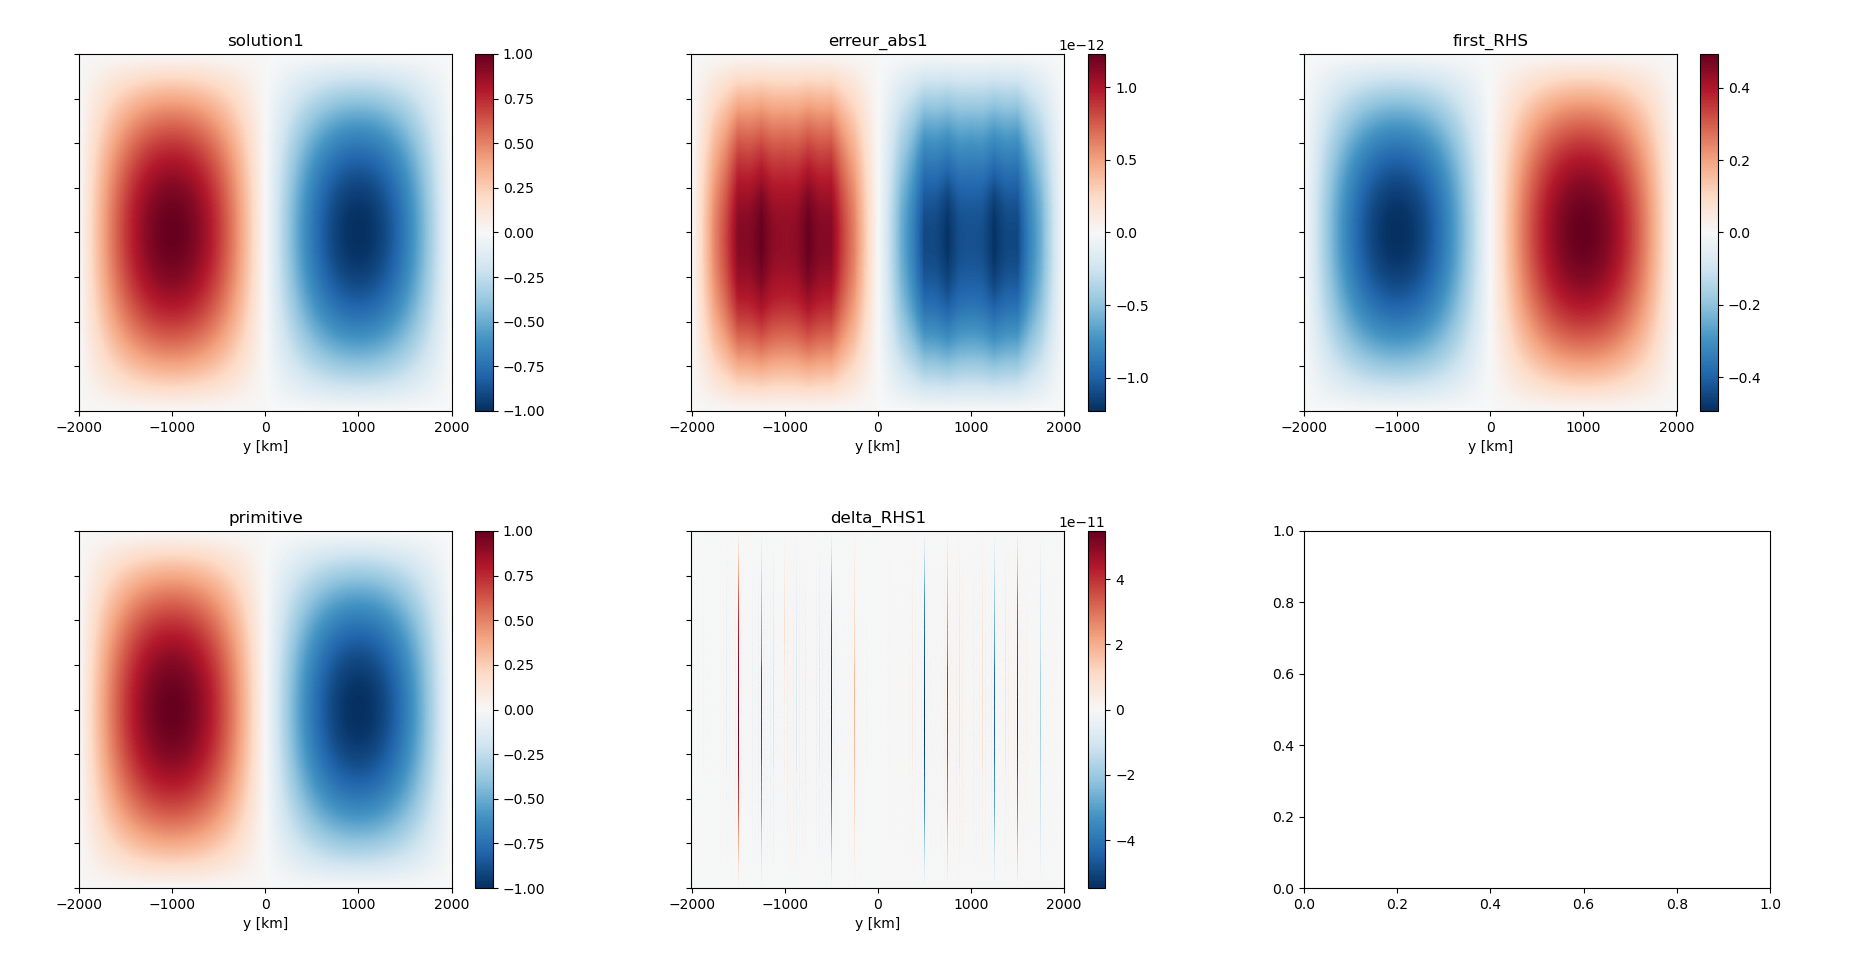
\includegraphics[width=0.8\textwidth]{figures/fishpack/2023-08-29-fishtest.png}
\caption{\label{fig:orgf90a24b}Comparaison des mêmes quantités évaluées avec MUDPACK, mais avec le solveur Fishpack. Résultat ahurissant.}
\end{figure}

Ce lundi soir et mardi, j'étais un peu épuisé qu'on perde autant de temps sur \emph{MUDPACK}, c'est pourquoi j'ai commencé à regarder ailleurs.
Entre autre, un article en ligne comparait l'efficacité de trois méthodes pour solutionner rapidement les équations différentielles partielles du genre de celle à laquelle on a affaire (équation \ref{eq:orgff87505}).\bigskip

Concrétement, \emph{MUDPACK} était la moins bonne, mais il mentionnait un autre module nommé \emph{fishpack}.
Donc, je me suis lancé.
Deux versions existaient en ligne, soit celle de NCAR et une \href{https://github.com/jlokimlin/fishpack}{version mise à jour} il y a 6 ans.
Bien entendu j'ai pris la plus récente pour m'assurer qu'on puisse utiliser les type DOUBLE PRECISION.\bigskip

Après une journée de travail, j'en suis arrivé à la figure \ref{fig:orgf90a24b}.
Le résultat est ahurissant, on obtient une erreur absolue de l'ordre de \(10^{-12}\) et un écart de \(\zeta\) de \(10^{-11}\).
On peut en déduire de \emph{MUDPACK} est complétement surclassé.
Sans oublier que le temps de calcul est minimal aussi.

\subsection{Implémentation dans le modèle en eau peu profonde -- \textit{<2023-08-30 Wed>}}
\label{sec:org55c145c}

Comme au premier jet, nous solvons l'équation \ref{eq:orgff87505} directement.
Donc, aucun besoin de corriger le RHS ou l'écart entre les deux champs : on corrige directement le champ courant (donc celui mis à jour : \(ilevel=3\)).
Si le besoin pour une meilleure précision se fait sentir, on pourra revenir à nos bonnes habitudes de seulement corriger l'écart entre les champs \(ilevel=1\) et \(ilevel=3\), de sorte à suivre le pas de temps de type \emph{leapfrog}.

\subsubsection{Rappel de l'analyse dimensionelle associée au vent \textit{<2023-08-31 Thu>}}
\label{sec:orgecfebd0}
La nuit dernière, j'ai lancé une simulation de 10 ans, mais nous sommes toujours dans le \emph{spin up}.
Après un peu de débroussaillage, j'ai vu que ça venait probablement du \(\tau\) insuffisant.,
À la base, j'avais mis ça car David voulait voir le système évoluer sans les termes non-linéaires et je l'avais oublié là.
J'ai relancé la simulation avec un vent de \(\tau = 0.1 Nm^{-2}\).\bigskip

Les paramètres sont illustrés dans le tableau \ref{tab:orge1e9d0c}.

\begin{table}[htbp]
\caption{\label{tab:orge1e9d0c}Paramètres utilisés dans la simulation de jeudi matin (\textit{<2023-08-31 Thu>}).}
\centering
\begin{tabular}{llrl}
\hline
\hline
Paramètres & Symbole & Valeur & Unité\\[0pt]
\hline
Taille du domaine & L\textsubscript{x} = L\textsubscript{y} & 2000 & km\\[0pt]
Nombre de points de grilles & nx = ny & 513 & --\\[0pt]
Pas de temps & \(\Delta\) t & 300 & s\\[0pt]
Paramètre de Coriolis & f & 7\texttimes{}10\textsuperscript{-5} & s\textsuperscript{-1}\\[0pt]
Paramètre beta & beta & 1\texttimes{}10\textsuperscript{-11} & m\textsuperscript{-1}s\textsuperscript{-1}\\[0pt]
Amplitude du vent & \(\tau\)\textsubscript{atm} & 0.1 & N m\textsuperscript{-2}\\[0pt]
Coefficient de visc. biharmonique & A\textsubscript{bh} & dx\textsuperscript{4} \texttimes{}10\textsuperscript{-5} & s\textsuperscript{-1}\\[0pt]
Coefficient de frottement & r\textsubscript{drag} & 10\textsuperscript{-7} & s\textsuperscript{-1}\\[0pt]
Vitesse des ondes internes barocliniques & c\textsubscript{bc} & 2 & ms\textsuperscript{-1}\\[0pt]
Épaisseur de la couche supérieure & H\textsubscript{1} & 1000 & m\\[0pt]
Épaisseur de la couche inférieur & H\textsubscript{2} & 3000 & m\\[0pt]
\hline
\end{tabular}
\end{table}

L'analyse dimensionnel va comme suit : Pour l'évolution,
\begin{equation}
   \pdv{\uu}{t} \Rightarrow \qty[ \frac{ms^{-1}}{s}] \Rightarrow \qty[\frac{m}{s^2}]. 
\end{equation}

Pour le terme associé au frottement visqueux du vent à la surface,
\begin{equation}
   \frac{\tau}{\rho h} \Rightarrow \frac{\qty[N m^{-2}]}{\qty[Kg\cdot m^{-3}] \qty[m]} \Rightarrow \qty[\frac{N}{Kg}] \Rightarrow \frac{\qty[Kg \cdot m s^{-2}]}{[Kg]} \Rightarrow \qty[\frac{m}{s^2}].
\end{equation}
Bonne nouvelle! Notre schéma pour le frottement visqueux à la surface est bon et je ne fais pas des erreurs stupides depuis 6 mois! \emph{Cheers!} \bigskip

Le test est réussi! Ça marche à merveille (voir figure \ref{fig:org7c77d1d}).

\begin{figure}[htbp]
\centering
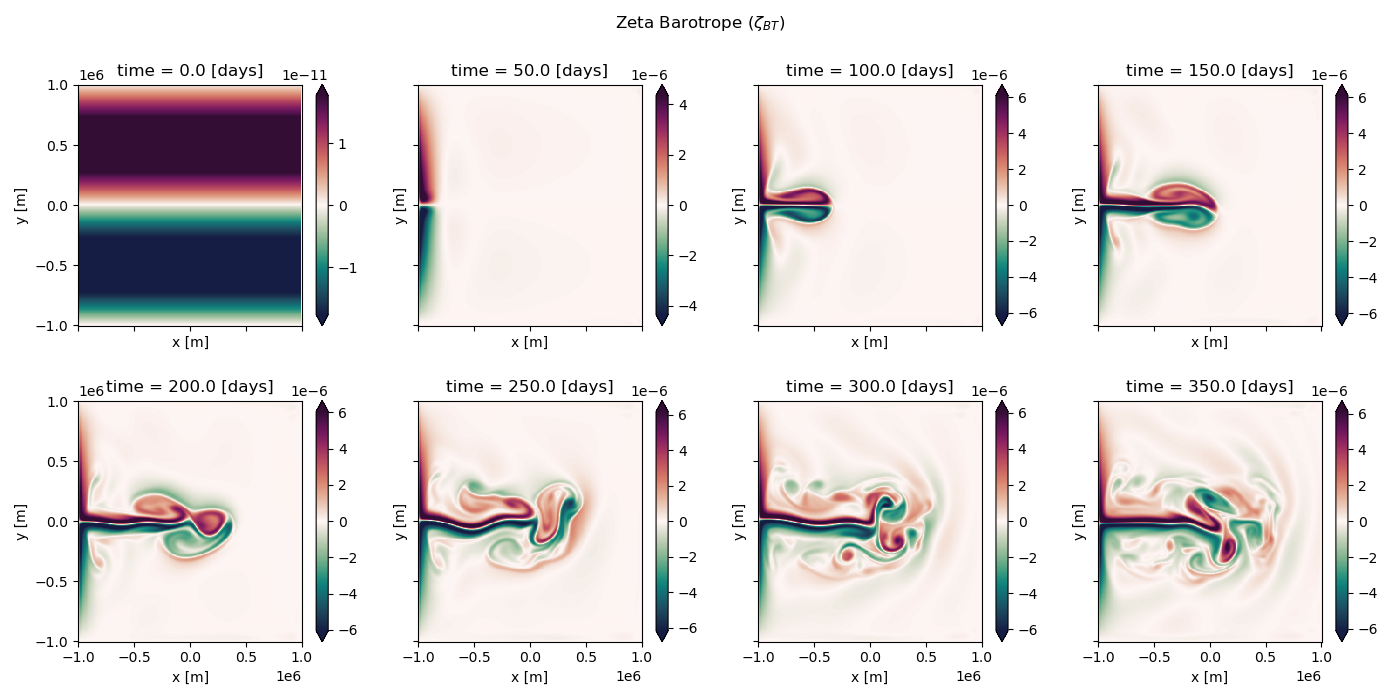
\includegraphics[width=.9\linewidth]{figures/tests/2023-09-06_8panneaux_zetaBT.png}
\caption{\label{fig:org7c77d1d}« Snapshots » (ou figures instantanées) de la vorticité barotrope calculée sur le domaines à différents moments. On voit apparaître les doubles gyres de Stommel.}
\end{figure}

\section{Modes baroclines pour l'étude des ondes de Rossby -- \textit{<2023-09-05 Tue>}}
\label{sec:orgc509b9c}

Dans un \href{rapport-2023-04-07.pdf}{rapport précédent}, nous avions utilisé le module \emph{LAPACK} pour retrouver les rayons de déformation de Rossby.
Le cadre théorique autour de la matière ce retrouve dans le \href{rapport-2023-03-24.pdf}{rapport de la fin du mois de mars}.
Finalement, encore d'autres éléments théoriques ont été amenés dans le \href{rapport-2023-03-31.pdf}{dernier rapport de mars}.\bigskip


\begin{wrapfigure}[12]{l}{0.35\textwidth}
\begin{center}
\vspace{-\baselineskip}
\begin{tikzpicture}
% Fond : 
\fill[blue!5] (0, 0) rectangle (4,-1);
\fill[blue!12] (0,-1) rectangle (4,-3);
% Lignes 
\draw [ultra thick] (0,0) node [anchor=east] {$\eta_1 = 0$} -- (4,0);
\draw [dotted] (0,-1) -- (4,-1);
\draw [ultra thick] (0,-3) node [anchor=east] {$\eta_B = 0$} -- (4,-3);
% Courbes : 
\draw [ultra thin] (0,-1.2) node [anchor=east] {$\eta_2\pt ,\ g'\pt$} sin (1.2,-0.8) cos (2,-1) sin (2.8,-1.2) cos (4,-0.8);
% Textes : 
\draw (2,0) node [anchor=south] {Surface fixe} ;
\draw (2,-3) node [anchor=north] {Plancher océanique} ;
% H-k
\node at (4.3,-0.5) (H1) {$H_1$};
\node at (4.3,-2) (H2) {$H_2$};
% d-k
\node at (2,-0.5) (d1) {$d_1$};
\node at (2,-2) (d2) {$d_2$};
% flèches 
\draw[>=stealth, ->|] (H1) -- (4.3, 0); 
\draw[>=stealth, ->|] (H1) -- (4.3,-1);
\draw[>=stealth, -> ] (H2) -- (4.3,-1); 
\draw[>=stealth, ->|] (H2) -- (4.3,-3);
\end{tikzpicture}
\end{center}
\caption{\label{orgb5c3e2c}Illustration d'un modèle \textit{shallow water} à deux couches (\(n_k = 2\)).}
\end{wrapfigure}

En premier lieu, dans un milieu continu linéarisé autour d'un courant moyen (ce qu'on appelle généralement un \emph{background flow}), l'équation d'évolution pour la vorticité potentielle quasi-géostrophique (QGPV) est donnée par
\begin{equation}
\label{eq:orgd7cb03e}
   \pdv{}{t} \qty[\laplacian\psi + \qty(\frac{f^2}{N^2})\pdv[2]{\psi}{z}] + \beta \pdv{\psi}{x} = 0.
\end{equation}
Comme point de départ, reprenons le système d'équations en eau peu profonde discrétisé en deux couches (\emph{Shallow Water Quasi-Geostrophic} abbrévé par \emph{SWQG}), soit
\begin{subequations}
\label{eq:orgc26fb2e}
\begin{align}
   &\pdv{}{t} \qty[\laplacian\psi_1 + \qty(\frac{f_0^2}{g'H_1}) \pt(\psi_2 - \psi_1)] + \beta \pdv{\psi_1}{x} = 0,\\
   &\pdv{}{t} \qty[\laplacian\psi_2 + \qty(\frac{f_0^2}{g'H_2}) \pt(\psi_1 - \psi_2)] + \beta \pdv{\psi_2}{x} = 0.
\end{align}
\end{subequations}

Nous avons devant nous un système d'équations couplées.
Notre objectif sera de trouver une base de \(\boldsymbol{\psi}\) qui \textbf{découple} ces deux équations.
Par inspection (et traditionnellement) (voir \citep[p.230]{vallis_2006}, on peut poser deux combinaisons linéaires, soit
\begin{align}
   &&\hat{\psi} = \psi_1 - \psi_2 ,&& \bar{\psi} = \frac{H_1\psi_1 + H_2\psi_2}{H_1+H_2}, &&
\end{align}
où \(\hat{\psi}\) est la solution dite \textbf{barocline} et \(\bar{\psi}\) est la solution dite \textbf{barotrope}.
Après un peu d'algèbre, on se retrouve avec le système d'équations
\begin{subequations}
\begin{align}
   &\pdv{}{t} \laplacian\bar{\psi} + \beta \pdv{\bar{\psi}}{x} = 0,\\
   &\pdv{}{t} \qty[\laplacian\hat{\psi} + \frac{1}{L_R^2}\hat{\psi}] + \beta \pdv{\hat{\psi}}{x} = 0,
\end{align}
\end{subequations}
où \(L_R\) est le rayon de déformation de Rossby qui est définit par
\begin{align}
   && L_R \equiv \frac{f_0}{\sqrt{g'\hat{H}}}, && \hat{H} = \frac{H_1H_2}{H_1+H_2}.&&
\end{align}

\subsection{Décomposition à l'aide du problème au valeurs propres -- \textit{<2023-09-05 Tue>}}
\label{sec:orgb3b920d}

Ok, la méthode traditionnelle est \emph{bin correct}, mais elle ne fonctionne pas pour plusieurs couches.
Dans un problème à plusieurs couches, il faudrait trouver une base de solutions qui découplent les équations précédentes -- ce qui est essentiellement la description du problème aux valeurs propres.
En solvant l'équation caractéristique \ref{eq:orgc32049b}, on trouve justement une base qui solutionne notre système d'équations linéaires, donc qui trouve une base de solutions.
Commençons par poser le problème, soit
\begin{align}
   && f_1 = \frac{f_0^2}{g'H_1} && \text{et} && f_2 = \frac{f_0^2}{g'H_2}. &&
\end{align}

On peut alors prendre l'opérateur linéaire décrivant la stratification : \(\mathscr{L} = \qty(\frac{f^2}{N^2})\pt\pdv[2]{\psi}{z}\) et trouver une base de vecteurs propres qui \textbf{découplent} le système d'équations \ref{eq:orgeaa7570}.
Construisons la matrice \(A\), soit
\begin{align}
\label{eq:orgc32049b}
&& \mathscr{L} \pt\qty[ \hat{\psi} ] = \qty(\frac{f^2}{N^2})\pt\pdv[2]{}{z} \pt\qty[\hat{\psi}]= 
   \underbrace{
   \begin{pmatrix}
     -f_1 & +f_1 \\
     +f_2 & -f_2 \\
   \end{pmatrix}}_{A}
   \begin{pmatrix}
     \psi_1 \\
     \psi_2 \\
   \end{pmatrix}
   && \Longrightarrow
   && \boxed{ A \hat{\psi}^i = \lambda_i \hat{\psi}^i. } &&
\end{align}

\subsubsection{Rafraîchissement rapide sur le problème aux valeurs propres -- \textit{<2023-09-05 Tue>}}
\label{sec:orga8c6ec1}

C'est un problème aux valeurs propres, donc on peut créer l'équation charactéristique
\begin{align}
\label{eq:orgb3e9d6c}
   && A \vv^i = \lambda_i \vv^i && B \vv_i = (A - \lambda_i I)\vv^i = 0 &&
\end{align}
N'oublions pas que par définition, les vecteurs propres doivent être normalisés, de sorte que
\begin{equation}
   \vv^\dagger \vv = 1
\end{equation}
Et lorsque la matrice \(A\) est normale (\(AA^\dagger = A^\dagger A\)), la matrice \(B\) est aussi normale (voir le livre \citet*[p.274 pour un résumé sans précédent]{riley_hobson_bence_2006} pour une explication sans précédent).
\begin{proof}
La preuve est simple, 
\begin{equation}
   B\vv = 0 \ \Rightarrow\ (B\vv)^\dagger = \vv^\dagger B^\dagger = 0. 
\end{equation}
Ce qui nous permet de dire que
\begin{equation}
   \vv^\dagger B^\dagger B \vv = 0
\end{equation}
Si l'on réalise le produit $B^\dagger B$, on obtient
\begin{equation}
   B^\dagger B = (A-\lambda I)^\dagger (A-\lambda I) = A^\dagger A - \lambda^* A -\lambda A^\dagger + \lambda^*\lambda.
\end{equation}
Si la matrice $A$ est normale ($A^\dagger A = A A^\dagger$),
\begin{equation}
   B^\dagger B = A A^\dagger - \lambda^* A -\lambda A^\dagger + \lambda^*\lambda = BB^\dagger.
\end{equation}
Par conséquent, la matrice $B$ est aussi normale.
\end{proof}

Cette preuve est importante, car elle nous permet de démontrer que les vecteurs propres sont orthogonaux en prenant l'équation précédente.
Donc
\begin{equation}
   \vv^\dagger B^\dagger B \vv = \vv^\dagger BB^\dagger \vv = (B^\dagger \vv)^\dagger B^\dagger \vv = 0,
\end{equation}
d'où on en déduit que
\begin{equation}
   B^\dagger \vv = (A^\dagger -\lambda^* I ) \vv = 0.
\end{equation}
Par conséquent, les valeurs propres de la matrice \(A^\dagger\) sont données par le complexe conjugué des valeurs propres de la matrice \(A\). \bigskip

Ok, maintenant, prouvons que les vecteurs propres \(\vv\) sont orthogonaux si la matrice \(A\) est normale.
\begin{proof}
Prenons deux vecteurs propres qui satisfont l'équation [[eq:charac]], soient
\begin{subequations}
\begin{align}
   &A \vv^i = \lambda_i\vv^i;\\
   &A \vv^j = \lambda_j\vv^j.
\end{align}
\end{subequations}
On multiplie la seconde équation par $(\vv^i)^\dagger$,
\begin{align}
   & (\vv^i)^\dagger A\vv^j = \lambda_j(\vv^i)^\dagger\vv^j,\nonumber\\
   & (A^\dagger\vv^i)^\dagger\vv^j = \lambda_j(\vv^i)^\dagger\vv^j,\nonumber\\
   & (\lambda_i^*\vv^i)^\dagger\vv^j = \lambda_j(\vv^i)^\dagger\vv^j,\nonumber\\
   & (\lambda_i - \lambda_j) (\vv^i)^\dagger\vv^j = 0
\end{align}
Donc, à moins que $\lambda_i = \lambda_j$ (ce qui n'est pas le cas), les vecteurs $\vv^i$ et $\vv^j$ sont orthogonaux. \end{proof}

\subsubsection{Trouver les fonctions verticales baroclines dans le modèle SWQG à deux couches -- \textit{<2023-09-05 Tue>}}
\label{sec:orge40b696}

À moins que l'épaisseur des deux couches soit la même (\(f_1 = f_2\) donc \(H_1 = H_2\)), notre système d'équations couplées \ref{eq:orgc32049b} ne nous offrira pas vraiment une matrice normale à résoudre (donc \(AA^\dagger\not=A^\dagger A\)).
Par conséquent, les fonctions baroclines (ou nos vecteurs propres) ne seront pas orthogonaux (\(\hat{\psi}^i \cdot \hat{\psi}^j \not= 0\)).
Il est possible que les couches aillent la même épaisseur (ou la même stratification dans le problème à \(>2\) couches), mais ça ne sera jamais vraiment le cas.\bigskip

Utilisons la méthode précédente pour trouver les vecteurs propres de la matrice \(A\) (\ref{eq:orgc32049b}), soit
\begin{align}
   \begin{vmatrix}
     -f_1 - \lambda & f_1 \\
     f_2 & -f_2 - \lambda \\
   \end{vmatrix} = (f_1+\lambda)(f_2+\lambda) - f_1 f_2 = \lambda^2 + f_1 \lambda + f_2 \lambda + 0 =\boxed{ \lambda(\lambda + f_1 + f_2) = 0 }
\end{align}
On trouve donc deux valeurs propres, soient
\begin{subequations}
\begin{align}
   & \lambda_1 = 0, \\
   & \lambda_2 = - (f_1+f_2).
\end{align}
\end{subequations}

On reprend l'équation caractéristique, ce qui nous donne un système d'équation
\begin{equation}
   \begin{pmatrix}
     - f_1 v_1 & f_1 v_2 \\
     f_2 v_1 & -f_2 v_2 \\
   \end{pmatrix} = \lambda_i
   \begin{pmatrix}
     v_1\\
     v_2\\
   \end{pmatrix}
\end{equation}
Si \(\lambda = 0\), alors \(v_1 = v_2\) et le premier vecteur propre est donné par
\begin{equation}
   \boxed{\hat{\vv}^1 = \qty( \frac{1}{\sqrt{2}}\ ;\ \frac{1}{\sqrt{2}}).}
\end{equation}
Tandis que le second est donné par
\begin{align}
   \cancelto{0}{-f_1 v_1} + f_1 v_2 & = \cancelto{0}{-f_1 v_1} - f_2 v_1 \\
   f_2 v_1 - \cancelto{0}{f_2 v_2} & = -f_1 v_2 - \cancelto{0}{f_2 v_2} \\
\end{align}
donc
\begin{equation}
   \hat{\vv}^2 = \qty( \frac{f_1}{(f_1^2+f_2^2)^{1/2}},\ \frac{-f_2}{(f_1^2+f_2^2)^{1/2}})\ \Longrightarrow \hspace{0.2cm}\boxed{\hspace{0.2cm}\hat{\vv}^2=\qty( \frac{H_2}{(H_1^2+H_2^2)^{1/2}},\ \frac{-H_1}{(H_1^2+H_2^2)^{1/2}})\hspace{0.2cm}}
\end{equation}

Mentionnons que c'est différent de ce que nous avions trouvé avec la méthode traditionnelle, je sais pas trop pourquoi\ldots{} anyway.\bigskip


\subsubsection{Résultats analytiquemes vs numériques -- \textit{<2023-09-06 Wed>}}
\label{sec:org6b5bdf1}

Pour des paramètres de l'ordre de ceux dans le tableau suivant,

\begin{center}
\begin{tabular}{llrl}
\hline
\hline
Paramètres & Symbole & Valeur & Unité\\[0pt]
\hline
Paramètre de Coriolis & f\textsubscript{0} & 7\texttimes{}10\textsuperscript{-5} & s\textsuperscript{-1}\\[0pt]
Paramètre beta & beta & 1\texttimes{}10\textsuperscript{-11} & m\textsuperscript{-1}s\textsuperscript{-1}\\[0pt]
Épaisseur de la couche supérieure & H\textsubscript{1} & 1000 & m\\[0pt]
Épaisseur de la couche inférieur & H\textsubscript{2} & 3000 & m\\[0pt]
Nombre de couches & nz & 2 & [--]\\[0pt]
\hline
\end{tabular}
\end{center}

on retrouve deux vecteurs propres analytiquement, soient
\begin{subequations}
\begin{align}
   & \hat{\vv}^1 = \qty(0.707106769,\ \hspace{0.2cm} 0.707106769\pt) \\
   & \hat{\vv}^2 = \qty(0.948683298,\ - 0.316227766)
\end{align}
\end{subequations}

Et lorsqu'on les compare avec ceux calculés numériquement à l'intérieur de la sous-routine d'initialisation du modèle \emph{shallow water} pour deux couches, on retrouve les mêmes vecteurs propres dans la figure \ref{fig:orgcb51035}.
Donc, il faut en conclure que notre implémentation à nz couches (voir section \ref{org08d342e} pour comprendre comment on résoud le cas à nz couches) fonctionne aussi pour 2 couches.

\begin{figure}[htbp]
\centering
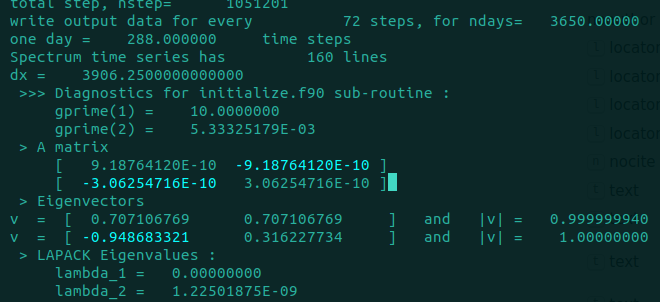
\includegraphics[width=.9\linewidth]{figures/vallis/eigenvalues.png}
\caption{\label{fig:orgcb51035}« Screenshot » des diagnostiques d'algèbre linéaire de LAPACK.}
\end{figure}
\newpage
\subsection{Fonctions baroclines du cas à plusieurs couches -- \textit{<2023-09-06 Wed>}}
\label{sec:org75b8898}
\label{org08d342e}

\begin{wrapfigure}{r}{0.5\textwidth}
\begin{center}
\vspace{-2\baselineskip}
\begin{tikzpicture}[scale=1.1]
% Fond : 
\fill[blue!5] (0, 0) rectangle (4,-1);
\fill[blue!8] (0,-1) rectangle (4,-2);
\fill[blue!11] (0,-2) rectangle (4,-3);
\fill[blue!14] (0,-3) rectangle (4,-4);
% Lignes 
\draw [ultra thick] (0,0) node [anchor=east] {$\eta_1 = 0$} -- (4,0);
\draw [dotted] (0,-1) -- (4,-1);
\draw [dotted] (0,-2) -- (4,-2);
\draw [dotted] (0,-3) -- (4,-3);
\draw [ultra thick] (0,-4) node [anchor=east] {$\eta_B = 0$} -- (4,-4);
% courbes : 
\draw [ultra thin] (0,-1.2) node [anchor=east] {$\eta_2$} sin (1.2,-0.8) cos (2,-1) sin (2.8,-1.2) cos (4,-0.8);
\draw [ultra thin] (0,-2.2) node [anchor=east] {$\eta_3$} sin (1.2,-1.8) cos (2,-2) sin (2.8,-2.2) cos (4,-1.8);
\draw [ultra thin] (0,-3.2) node [anchor=east] {$\eta_4$} sin (1.2,-2.8) cos (2,-3) sin (2.8,-3.2) cos (4,-2.8);
% Textes : 
\draw (2,0) node [anchor=south] {Surface fixe} ;
\draw (2,-4) node [anchor=north] {Plancher océanique} ;
% H-k
\node at (4.3,-0.5) (H1) {$H_1$};
\node at (4.3,-1.5) (H2) {$H_2$};
\node at (4.3,-2.5) (H3) {$H_3$};
\node at (4.3,-3.5) (H4) {$H_4$};
% d-k
\node at (2,-0.5) (d1) {$h_1$};
\node at (2,-1.5) (d2) {$h_2$};
\node at (2,-2.5) (d3) {$h_3$};
\node at (2,-3.5) (d4) {$h_4$};
% flèches 
\draw[>=stealth, ->|] (H1) -- (4.3, 0); 
\draw[>=stealth, ->|] (H1) -- (4.3,-1);
\draw[>=stealth, -> ] (H2) -- (4.3,-1); 
\draw[>=stealth, ->|] (H2) -- (4.3,-2);
\draw[>=stealth, -> ] (H3) -- (4.3,-2); 
\draw[>=stealth, ->|] (H3) -- (4.3,-3);
\draw[>=stealth, -> ] (H4) -- (4.3,-3); 
\draw[>=stealth, ->|] (H4) -- (4.3,-4);
\end{tikzpicture}
\end{center}
\caption{\label{org7999f60}Modèle « shallow water » à 4 couches.}
\end{wrapfigure}

Dans le cas à plusieurs couches, l'opérateur linéaire de flottabilité (\(\mathscr{L}\pt[\psi]\)) est représenté comme un ratio des variations verticales (\(\eta_{top},\ \eta_{bottom}\) : comme on peut voir à l'équation \ref{eq:orgeaa7570}) -- ou de \(h_i\) car c'est en fait un terme de «stretching» associé à la conservation de la vorticité.
\begin{equation}
   h_i = H_i + \eta_i - \eta_{i+1}.
\end{equation}

Notons que cette démarche avait déjà été réalisée dans le \href{rapport-2023-03-31.pdf}{rapport final de mars}, mais nous effectuons un rappel ici-bas car j'ai tout simplement tout oublié.
Pour toute définition, le lecteur est invité à se référer à la figure \ref{org7999f60}. \bigskip

Concrétement, l'équation de conservation de la vorticité potentielle en \emph{shallow water} (SWQG) dans chaque couche \citep[p.186]{vallis_2006} est trouvée en étandant la définition de l'équation continue \ref{eq:orgd7cb03e} à un domaine à différences finies.
Il en résulte l'équation
\begin{equation}
\label{eq:orgeaa7570}
   \pdv{}{t} \Bigg[ \laplacian{\psi^2_k} + \underbrace{\qty(\frac{f_0^2}{g_k' H_k})\pt \overbrace{\qty(\psi_{k-1}-\psi_k)\grande}^{\eta\pt(top)} -\pt \qty(\frac{f_0^2}{g_{k+1}' H_k})\pt \overbrace{\qty(\psi_{k} - \psi_{k+1})\grande}^{\eta\pt(bottom)}}_{\mathscr{L \psi}} \Bigg] + \beta\pt \qty(\pdv{\psi_k}{x}) = 0.
\end{equation}

Plus clairement,
\begin{equation}
   \pdv{}{t} \Bigg[ \laplacian{\psi^2_k} + \underbrace{\qty(\frac{f_0^2}{g_k' H_k})\pt \psi_{k-1} - \qty(\frac{f_0^2}{g_k' H_k} + \frac{f_0^2}{g_{k+1}' H_k}) \pt \psi_{k} - \qty(\frac{f_0^2}{g_{k+1}' H_k})\psi_{k+1}}_\mathscr{L\psi} \Bigg] + \beta\pt \qty(\pdv{\psi_k}{x}) = 0.
\end{equation}

Si l'on découple les partie horizontales et verticales de nos fonctions de courant, de sorte que
\begin{equation}
   \psi(x,y,z,t) = \tpsi(z) \cdot\exp{i\pt(k_x x + k_y y -\omega t)},
\end{equation}
l'opérateur linéaire vertical de flottabilité « \(\mathscr{L}\pt[\tpsi_k\pt]\) » est ainsi décrit par l'expression
\begin{equation}
\boxed{\hspace{0.4cm}
\mathscr{L}\pt[\tpsi_k] = \qty( F_{(k,k+1)} + F_{(k,k)}) \ \tpsi_k
- F_{(k,k)}\ \tpsi_{k-1}
- F_{(k,k+1)}\ \tpsi_{k+1},
\hspace{0.5cm}\text{où}\hspace{0.5cm}
F_{(i,j)} = \frac{f_0^2}{H_i g'_j},
\hspace{0.4cm} }
\end{equation}
et où \(g'_i\) est la gravité réduite à la surface d'une couche, donc
\begin{equation}
g_k' = g \pt\qty(\frac{\rho_k - \rho_{k-1}}{\rho_1}).
\end{equation}
Mentionnons que les valeurs sont négatives, car on définit le problème aux valeurs propres comme
\begin{equation}
   \mathscr{L}\pt [\hat{\psi}] + \Gamma_k\hat{\psi} = 0,
\end{equation}
comme mentionné dans le livre de \citet*[p.469]{vallis_2006}. \bigskip

En terme de matrice, l'opérateur linéaire de flottabilité s'exprime par
\begin{equation}
\overbrace{
\begin{pmatrix}
   F_{(1,2)} + F_{(1,1)} & -F_{(1,2)}           & 0           & \cdots   &  0 \\
   -F_{(2,2)}           & F_{(2,3)} + F_{(2,2)} & -F_{(2,3)}   & \cdots   &   0 \\
   \vdots             & \vdots             & \vdots      & \ddots   &  \vdots \\
   0                  & \cdots             & 0           & -F_{(nz,nz)} & F_{(nz,nz+1)} + F_{(nz,nz)} \\
\end{pmatrix}}^A
\begin{pmatrix}
   \tpsi_1    \\
   \tpsi_2    \\
   \vdots     \\
   \tpsi_{nz} \\
\end{pmatrix}
+ \Gamma_k
\begin{pmatrix}
  \tpsi_1    \\
  \tpsi_2    \\
  \vdots     \\
  \tpsi_{nz} \\
\end{pmatrix} = 0
\end{equation}

Les vecteurs propres ainsi trouvé à l'aide de la décomposition \(\hat{\psi}^i\) formeront une \textbf{base non-orthogonale} étant donné que la matrice \(A\) n'est pas dite « normale » (\(A^\dagger A = A A^\dagger\)).
La matrice \(A\) est seulement normale lorsque la stratification est constante, donc lorsque
\(N^2\) est pareil sur toute la colonne d'eau.
Mentionnons que le cas analytique à 3 couches identiques a d'ailleurs déjà été résolue analytiquement dans le \href{rapport-2023-04-07.pdf}{rapport du début d'avril}, donc je ne le referais pas ici.
J'en ai déjà beaucoup trop refait\ldots{}

\section{Implémentation fonctions barotropes}
\label{sec:orgf7da563}
Avant tout, rappellons que la décomposition de Helmholtz est définie par
\begin{subequations}
\begin{align}
   \uu &= -\gradient{\phi} + \kvf \times \gradient{\psi},\\
   \divergence{\uu} &= -\laplacian{\phi},\\
   \kvf\cdot\curl{\uu} &= \laplacian{\psi}.
\end{align}
\end{subequations}
Donc, on peut trouver la fonction de courant \(\psi(k)\) en solvant l'équation précédente à l'aide de Fishpack.
Comme les fonctions baroclines verticales ont été définies précédemment \(\hat{\psi}\), on trouve les modes baroclines à l'aide de
\begin{align}
   &&\psi_\text{mode}^i = \sum_k^{nz} \hat{\psi}^i(k)\cdot  \psi_k(x,y),
   &&\zeta_\text{mode}^i = \sum_k^{nz} \hat{\psi}^i(k)\cdot  \zeta_k(x,y).&&
\end{align}

\bibliography{/home/charlesedouard/Desktop/Travail/Documentation/master-bibliography}
\end{document}